\Chapter{Az alkalmazás tervezése}

Az általam készített alkalmazás célja egy olyan darts-os webes alkalmazás létrehozása amellyel saját versenyeket tudunk létrehozni a tetszésünk szerinti beállításokkal. A mérkőzések adatait a játékosok rögzítik egy pontszámláló segítségével, lehetőleg a mérkőzés valós lejátszásával párhuzamosan. Az oldal ezekből az adatokból állít elő statisztikákat a mérkőzésekről, a játékosokról és a versenyekről.


Ebben a fejezetben az implementáció nem kell, hogy túl nagy szerepet kapjon.
Ez még csak a tervezési fázis.
(Nyilván ha olyan a téma, hogy magának az implementációnak a módjával foglalkozik, adott formális nyelvet mutat be, úgy a kódpéldákat már innen sem lehet kihagyni.)

\Section{Fő komponensek}
\begin{itemize}
\item Jól átlátható és átjárható oldalak
\item Több féle verseny létrehozása
\item Versenyek, lejátszása
\item Szűrési lehetőségek (Játékos, Verseny, Statisztikai szempont, stb.)
\item Keresési lehetőségek (Játékos, Verseny)
\item Aktív és már befejezett versenyek nyilvántartása és kezelése
\item Mérkőzések lejátszása
\item Mérkőzés, játékos és verseny adatlapok megjelenítése
\item Mérkőzés, játékos és verseny statisztikák feldolgozása és megjelenítése
\item Felhasználói bejelentkezés/regisztráció
\item Felhasználói adatlap kezelése

\end{itemize}

Táblázatokhoz a \texttt{table} környezetet ajánlott használni.
Erre egy minta \aref{tab:minta}. táblázat.
A hivatkozáshoz az egyedi \texttt{label} értéke konvenció szerint \texttt{tab:} prefixszel kezdődik.

\begin{table}[h]
\centering
\caption{Minta táblázat. A táblázat felirata a táblázat felett kell legyen!}
\label{tab:minta}
\begin{tabular}{l|c|c|}
a & b & c \\
\hline
1 & 2 & 3 \\
4 & 5 & 6 \\
\hline
\end{tabular}
\end{table}

\Section{Statisztikai opciók és számításuk bemutatása}
Mint minden sportban, a dartsban is a mérkőzésekből különböző statisztikai adatok nyerhetők ki, az átlagoktól kezdve, a 180as dobások számán át, a kiszálló dobások hatékonyságáig. Az alkalmazás fő funkciója, hogy egy adatbázisból, - amely meccsenként tartalmazza az adott meccshez tartozó dobásokat- , kiszámítja a statisztikákat. A statisztikák nem csupán mérkőzésenként kerülnek kiszámításra és megjelenítésre, hanem elérhetőek játékosonként is ahol egy adott játékosnak az adatbázisban lévő összes mérkőzése kerül számításba.

Az alábbi pontokban azok a statisztikai elemek szerepelnek amelyek kiszámításra kerülnek a meccsek vagy a játékosok esetében.

\begin{itemize}
\item Nyert szettek és/vagy legek száma:

Magának az eredmények a megjelenítése. Olyan mérkőzések esetében, amelyeket szettekre játszanak, külön megjelenítésre kerülnek az adott szettben megnyert legeknek a száma is. Egy leget az a játékos nyeri akinek a pontszámát a legkevesebb nyílból sikerül 0-ra redukálnia.
\item Átlagok:

Egy játékos átlagát legenként/szettenként számoljuk ki a körönként dobott pontszámok szummázásával, amelyet elosztunk a körök számával.
\item Kiszálló dobások hatékonysága:
A kiszálláshoz szükséges duplára sikeresen eldobott nyilak és a kiszállóhoz szükséges duplára összesen eldobott nyilak arányát mutatja.
\item 180-as dobások száma:

Azon dobások száma játékosonként, amely elérte az egy körben dobható maximális pontszámot, azaz a 180-at.
\item 140 feletti dobások száma:

Azon dobások száma játékosonként, amelynek az értéke 140 vagy annál több, de kevesebb, mint 180.
\item 100 feletti dobások száma:

Azon dobások száma játékosonként, amelynek az értéke 100 vagy annál több, de kevesebb, mint 180.
\item Legmagasabb kiszálló:

Egy játkos legmagasabb pontszámú kiszállást is érő dobása egy meccsen.
\item Első 9 nyíl átlaga:

A játékos a mérkőzésben legenként eldobott első 9 nyilának az értékei szummázva és osztva a lejátszott legek számának háromszorosával.
\item Első 3 nyíl átlaga:

A játékos a mérkőzésen eldobott első 3 nyilának, azaz az első körének az értékei szummázva és osztva a lejátszott legek számával
\item Első, második és harmadik nyíl átlag értéke:

Egy játékos által körönként eldobott első, második és harmadik nyilak értékeinek az átlaga a teljes mérkőzésre/legre kivetítve.
\item Sikeres egy, kettő, és három nyilas kiszállók aránya:

Sikeresen bedobott 1, 2 és 3 nyilat igénylő kiszállóknak a száma elosztva az összes olyan kör számával, amikor a játékosnak esélye volt kiszállni.
\item Sikeresen bedobott meccs nyilak aránya:

Azon dupla szektorra sikeresen eldobott nyilaknak a száma, elosztva az összes olyan eldobott nyilaknak a számával amikor az adott játékosnak már egy nyíl is elég lett volna a mérkőzés megnyeréséhez.
\item Eltalált tripla 20-ak aránya:

Az összes olyan nyilaknak a száma amellyel az adott játékos sikeresen eltalálta a tripla 20-as szektort, elosztva minden 20-as szektorra dobott nyilak számával.
\item Elvesztett kezdések aránya:

Azon legeknek a száma amikor az adott játékos olyan leget vesztett el amely az ő dobásával kezdődött.
\item Legenként dobott 180-ak aránya:

Az adott játékos összes 180-al zárult körének a száma elosztva a lejátszott legek számával.

\end{itemize}


Ábrákat a \texttt{figure} környezettel lehet használni.
A használatára egy példa \aref{fig:cimer}. ábrán látható.
Az \texttt{includegraphics} parancsba 
Az ábrák felirata az ábra alatt kell legyen.
Az ábrák hivatkozásához használt nevet konvenció szerint \texttt{fig:}-el célszerű kezdeni.

\begin{figure}[h]
\centering

\includegraphics[scale=0.3]{images/me_logo.png}
\caption{A Miskolci Egyetem címere.}
\label{fig:cimer}
\end{figure}

\Section{Az oldalak bemutatása}
Az alkalmazás több oldalból tevődik össze, de természetesen az oldalak között egyszerű az átjárhatóság. Ez a fejlécnek köszönhető ahol a menüpontokban az összes oldal megtalálható és a fejléc természetesen minden oldalon elérhető.

Az oldal címére kattintva érhetjük el a kezdő oldalt, mellette pedig menüpontokban szerepelnek a felhasználói adatlap, a játékosok, a versenyek, és a rangsorok oldalaira irányító gombok. A versenyek a játékosok és a mérkőzések külön adatlapokat kaptak, amelyek szintén külön oldalon érhetőek el.
Az oldalakon található legtöbb információ linkelve van a hozzájuk tartozó oldallal.

\subsection{Nyitó oldal}
A nyitó oldallal mindig a weblap megnyitásakor találkozunk, ahol a már meglévő felhasználóknak lehetőségük van bejelentkezni az új felhasználók pedig egy regisztrációt követően tudnak belépni az alkalmazásba. A fent említett funkciók és oldalak csak ezt követően érhetőek el érvényes fiókkal rendelkező felhasználók számára.
Például egy mérkőzésre rákattintva annak az adatlapját érhetjük el, ahol minden a mérkőzéssel kapcsolatos adat és információ megtalálható a feldolgozott statisztikákkal együtt. Ugyanez igaz a játékosokra és a tornákra is, mivel ha a nevükre rákattintunk, akkor megjelenik az adott játékos vagy torna adatlapja.

\begin{figure}[h]
\centering
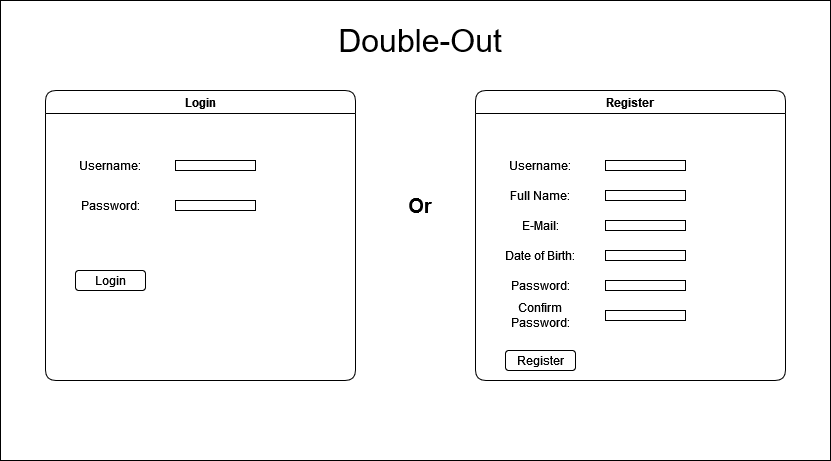
\includegraphics[scale=0.3]{images/LandingPage.drawio.png}
\caption{A nyitó oldal vázlata}
\label{fig:cimer}
\end{figure}

\subsection{Kezdő oldal}
A bejelentkezést követően a kezdő oldalon jelennek meg a még folyamatban lévő tornák külön blokkokban. A blokkban látható a torna neve a létrehozás időpontjával együtt, ezalatt kiírásra kerül még, hogy az adott torna jelenleg milyen fázisban jár és a mellette található „Countinue” gombbal a torna adatlapjára ugrunk, ahonnan folytatni tudjuk a tornát a hátralévő mérkőzések lejátszásával.

Amennyiben a felhasználó nem indított még tornát vagy csak éppen nincsen lezáratlan tornája, akkor ezek a blokkok nem jelennek meg. Azonban a kezdő oldalon megtalálható „+ New Tournament” gomb megnyomásával tudunk változtatni ezen az állapoton egy új torna létrehozásával. Itt minden szükséges adat kitöltésével létrehozható torna, amely a lezárásáig, vagy törléséig a korábban leírt módon már meg fog jelenni a kezdő oldalon is.

\begin{figure}[h]
\centering
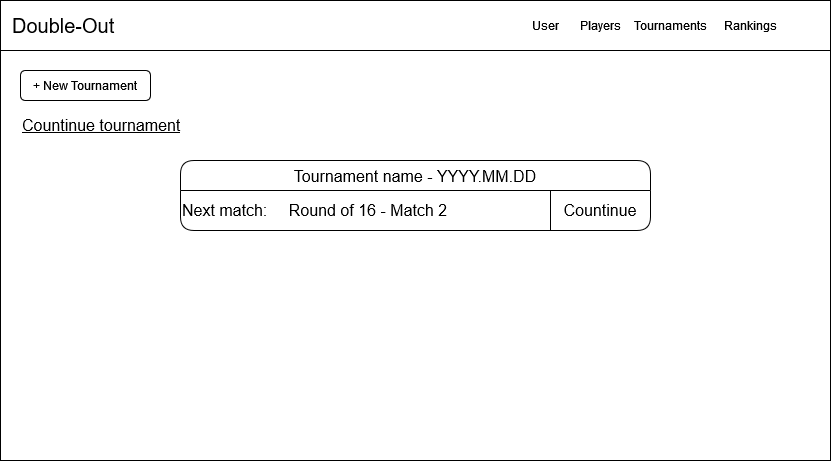
\includegraphics[scale=0.3]{images/HomePage.png}
\caption{A kezdő oldal vázlata}
\label{fig:cimer}
\end{figure}

\subsection{Versenyek oldala}
A versenyek oldalán tekinthetjük meg a még zajló és a már lezárult versenyeket is. A különböző versenyek külön blokkokban jelennek meg, ezek a blokkok pedig a versenyek egyes alap adatait tartalmazzák, mint például a nevüket, a létrehozás dátumát, valamint a verseny aktuális állapotát, azaz melyik a követkető forduló vagy befejezett verseny esetén a győztest. Az itt megtalálható „Countinue” vagy „Finished” gombokra kattintva az oldal tovább irányít minket a kiválasztott verseny adatlapjára.

A kezdőoldalhoz hasonlóan itt is megtalálható egy gomb az új versenyek létrehozásához amely a verseny létrehozás oldalára irányít át. 

\begin{figure}[h]
\centering
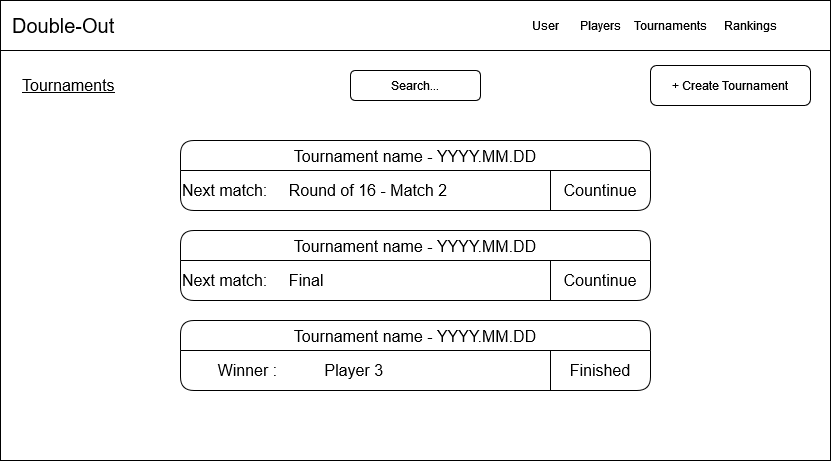
\includegraphics[scale=0.3]{images/TournamentsPage.png}
\caption{A versenyek oldalának vázlata}
\label{fig:cimer}
\end{figure}

\subsection{Verseny oldal}
A verseny oldalon a kiválasztott verseny adatlapját tekinthetjük meg. Az adatlap tartalmazza a már lejátszott mérkőzések eredményeit, illetve láthatjuk még a verseny lebonyolítása alapján hátralévő mérkőzéseket is. Ezen az oldalon láthatóak az adott verseny statisztikái is, amelyek a lejátszott mérkőzések statisztikái alapján kerülnek kiszámításra. Amennyiben egy versenyt nem kívánunk már nyilván tartan, akkor azt a „Delete Tournament” gombra kattintva törölhetjük az adatbázisból az állapotától (lejátszott vagy aktív) függetlenül.

\begin{figure}[h]
\centering
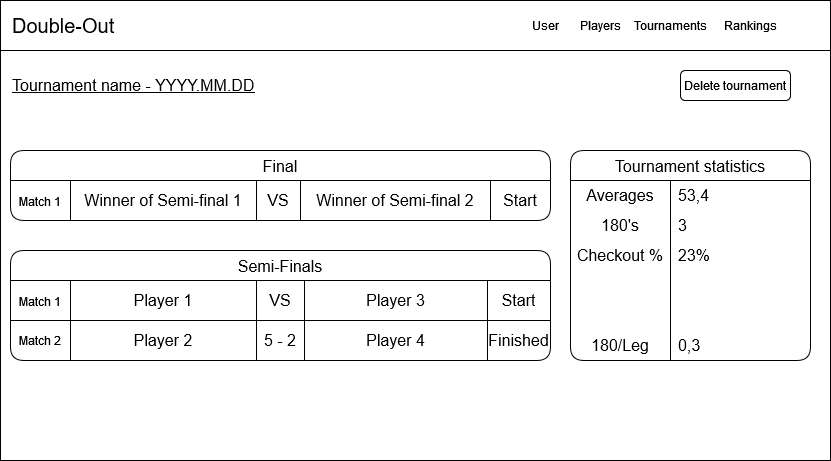
\includegraphics[scale=0.3]{images/TournamentPage.drawio(1).png}
\caption{A verseny oldal vázlata}
\label{fig:cimer}
\end{figure}

\subsection{Verseny létrehozása oldal}
A verseny oldalon megtekinthető a versenynaptár. A tornák az időpontjaik alapján kerülnek kilistázásra. Egy tornára rákattintva megtekinthetjük a torna adatlapját ahol további információk szerepelnek a tornáról illetve az eredményei is. Amennyiben még nem került idén megrendezésre az adott torna, akkor az előző évi eredményei is adatai jelennek meg.

\begin{figure}[h]
\centering
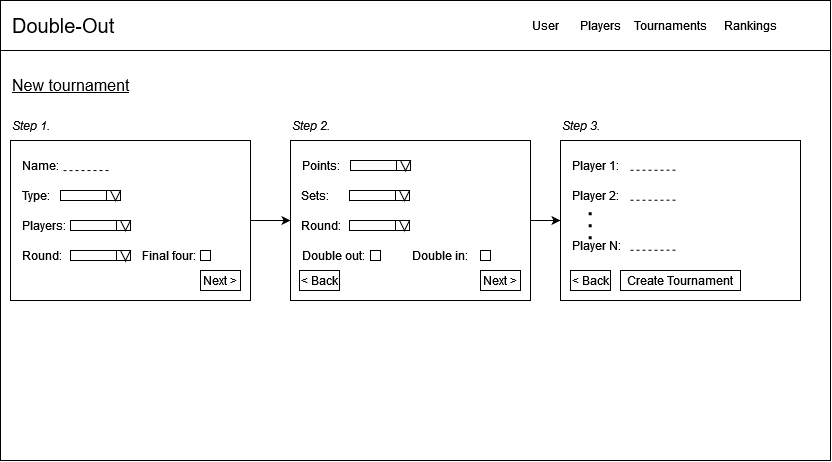
\includegraphics[scale=0.3]{images/CreateTournamentPage.drawio.png}
\caption{A verseny létrehozása oldal vázlata}
\label{fig:cimer}
\end{figure}

\subsection{Játékosok oldala}
A játékosok oldalán az alkalmazásban létrehozott versenyeken résztvevő játékosok találhatók meg, illetve a neveik alapján lehetőség van keresni is közöttük. Egy adott játékost kiválasztva a játékos adatlapját tudjuk elérni egy új oldalon.

\begin{figure}[h]
\centering
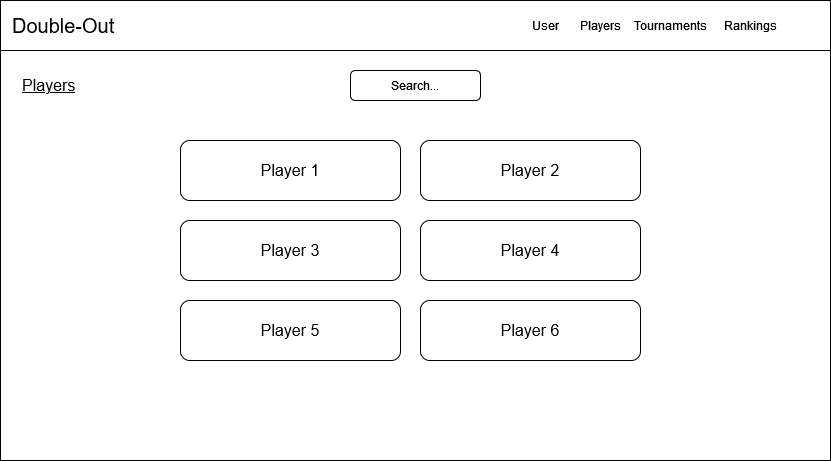
\includegraphics[scale=0.3]{images/PlayersPage.drawio.png}
\caption{A játékosok oldalának vázlata}
\label{fig:cimer}
\end{figure}

\subsection{Játékos oldal}
Minden játékos saját adatlappal rendelkezik, ahol az adott játékos statisztikáit tudjuk megtekinteni a már korábban is leírt szempontok szerint. Emellett a játékos eddigi verseny és mérkőzés mérlegét, vagyis a győzelmek és vereségek arányát. Végezetül pedig legutóbbi mérkőzéseinek az eredményeit is megtekinthetjük. Ezek az adatok folyamatosan frissülnek amennyiben a játékos újabb tornákon, illetve mérkőzéseken vesz részt.

\begin{figure}[h]
\centering
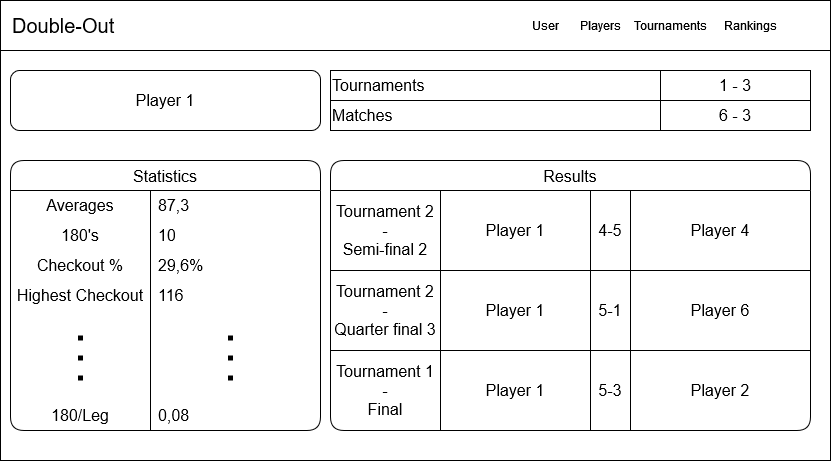
\includegraphics[scale=0.3]{images/PlayerPage.drawio.png}
\caption{A játékos oldal vázlata}
\label{fig:cimer}
\end{figure}

\subsection{Mérkőzés oldal}
A mérkőzés oldal tartalmazza a játékhoz szükséges pont kalkulátort amelybe a dobott pontokat tudjuk beírni az eltalált szektor és a szektoron belül eltalált terület megadásával, ezalapján kerül kiszámításra a dobás értéke ami a játék szabályai alapján kivonásra kerül a játékos pontjaiból és ez a folyamat addig ismétlődik amíg valamelyik meg nem nyeri a mérkőzést.

Ezekből a megadott adatokból kerülnek kiszámításra a statisztikák, amelyeket szintén ezen az oldalon tekinthetünk meg. A statisztikák „klasszikus” módon egy táblázatban jelennek meg, középen a statisztikai szempontok láthatóak tőle bal és jobb oldalra pedig a 2 játékos eredményei az adott statisztikai szempontban.

\begin{figure}[h]
\centering
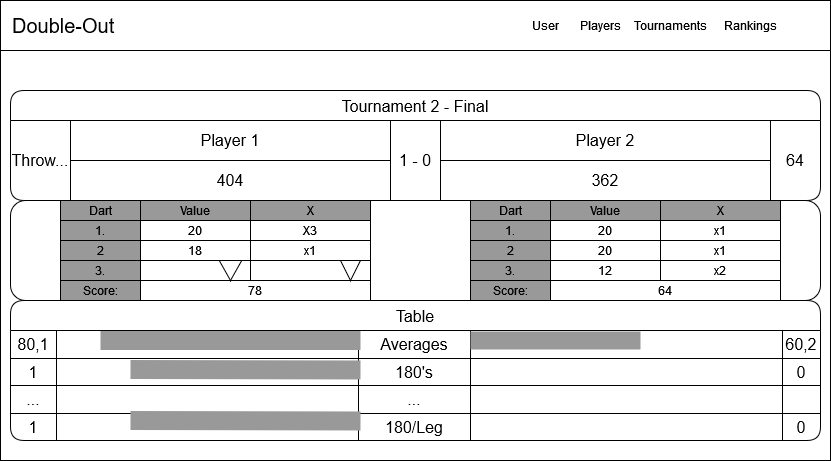
\includegraphics[scale=0.3]{images/MatchPage.drawio.png}
\caption{A mérkőzés oldal vázlata}
\label{fig:cimer}
\end{figure}

\subsection{Ranglisták oldala}
A ranglisták oldalán egy ranglista található, amely a versenyeken résztvevő játékosokat helyezi sorrendbe a különböző statisztikai szempontok alapján, illetve nem csak statisztikai szempontokra szűrhetünk, hanem az egyes versenyekre is.

\begin{figure}[h]
\centering
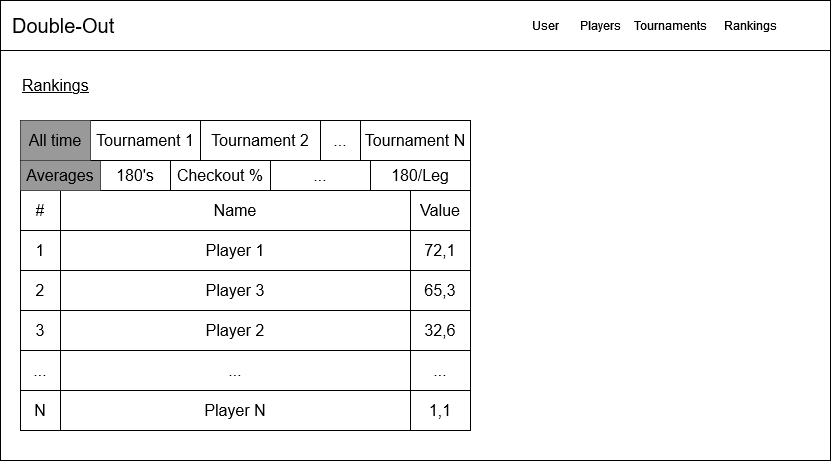
\includegraphics[scale=0.3]{images/Rankings.drawio.png}
\caption{A Ranglisták oldalának vázlata}
\label{fig:cimer}
\end{figure}

\subsection{Felhasználói adatlap oldala}
A felhasználói adatlap oldalát a sikeres bejelentkezés után tudjuk elérni. Itt megtekinthetőek a regisztrációkor megadott felhasználói adatok a jelszó kivételével. Az adatokat szerkeszteni is tudjuk a jelszóval együtt a profil szerkesztése menüpontban, ehhez szükséges a meglévő jelszó helyes megadása, ha ez a feltétel teljesült, akkor a módosítások sikeresen mentésre kerültek.

\begin{figure}[h]
\centering
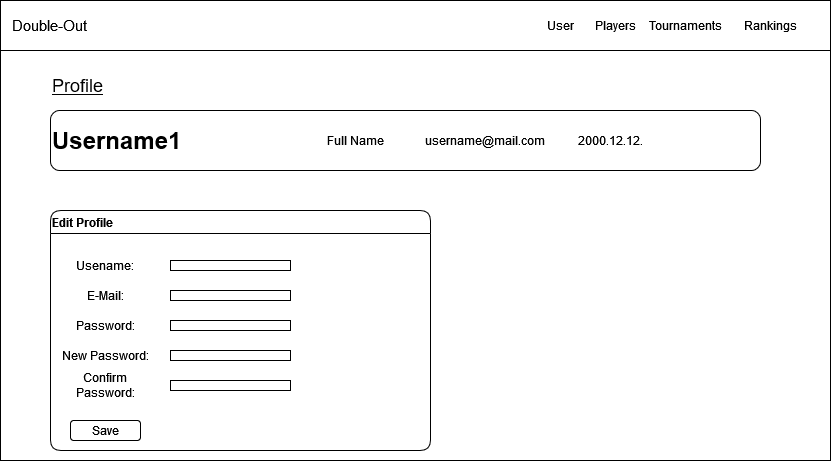
\includegraphics[scale=0.3]{images/ProfilePage.drawio.png}
\caption{A felhasználói adatlap oldalának vázlata}
\label{fig:cimer}
\end{figure}

\Section{Adatmodellek bemutatása}
A program megírása során külön adatmodelleket hoztam létre a játékosok, a versenyek, a mérkőzések, a statisztikák illetve a felhasználók számára. Az alkalmazás ezen adatmodellek alapján képes az adatok feldolgozására és azok küldésére az adatbázis számára, illetve fogadására is az adatbázis irányából. Az alábbi fastruktúra vázolja az alkalmazás felépítését az adatmodellek szempontjából. Egy felhasználó képes létrehozni egy versenyt, amely versenyből származnak a játékosok illetve a mérkőzések, az utóbbiból a statisztikák származnak, mivel azok a mérkőzés adatai alapján kerülnek kiszámításra. (MÉG MÓDOSÍTANI KELL AZ ÁBRA ALAPJÁN)

\subsection{Felhasználó adatmodell}
A felhasználó adatmodell a felhasználók adatainak a tárolására hivatott. A felépítés egyszerű, tartalmaz egy egyedi azonosítót, nevet, email címet, jelszót, illetve egy „isAdmin” és egy token adattagot. Az azonosítót az adatbázis generálja a létrehozáskor, a további adatokat pedig a regisztrációkor adjuk meg. A sikeres regisztráció után ezek az adatok mentésre kerülnek az adatbázisban és a későbbiekben már lehetősége lesz a felhasználónak bejelentkezni az oldalra ezen adatok megadásával.

\begin{cpp}
export const UserSchema = new Schema<User>({
    name: {type: String, required: true},
    email: {type: String, required: true, unique: true},
    password: {type: String, required: true},
    isAdmin: {type: Boolean, required: true},
}, {
    timestamps: true,
    toJSON:{
        virtuals: true
    },
    toObject:{
        virtuals: true
    }
});
\end{cpp}

\subsection{Verseny adatmodell}
A versenyek képezik az alkalmazáson belüli adatmodellek alapját, mivel a verseny létrehozásától függ a játékosok és mérkőzések létrehozása is. Az adatmodell tartalmazza a verseny azonosítóját, a nevét, a típusát a játékosok számát illetve 2 interfészt is, egyet a verseny mérkőzéseinek, az adatainak a beállítására és egyet a versenyben résztvevő játékosok megadására. A mérkőzések esetében meg kell adnunk, hogy hány pontosak lesznek a mérkőzések, hogy hány nyert leg-ig tart a mérkőzés, illetve, hogy duplával szükséges-e kiszállni. A játékosok esetében a résztvevők neveit kell csak megadni, vagyis annyi játékost amennyi a korábban megadott játékosok száma. A játékosok megadásánál lehetőségünk van új játékosok felvételére, illetve olyan játékosok felvételére is, akik korábban már vettek részt versenyben, vagyis már szerepelnek az adatbázisban.

\begin{cpp}
export const TournamentSchema = new Schema<Tournament>(
    {
        name:{type: String, required:true},
        type:{type: String, required:true},
        playersCount:{type: Number, required:true},
        match:
        [
            {
                points:{type: Number, required:true},
                legs:{type: Number, required:true},
                double_out:{type: Boolean, required:true},
            },
        ],
        players:
        [
            {
                name:{type: String, required:true},
            },
        ],
        currentRound:{type: String, required:true},
        winner:{type: String, required:false},
        runnerUp:{type: String, required:false},
    },{
        toJSON:{
            virtuals:true
        },

        toObject:{
            virtuals:true
        },
        timestamps:true
    }
);
\end{cpp}

\subsection{Játékos adatmodell}
A versenyeken résztvevő játékosok adatait a játékos adatmodell segítségével tároljuk. Ez az adatmodell is viszonylag egyszerű felépítésű, az adott játékos azonosítóját, a nevét illetve a verseny és mérkőzés mérlegét tárolja, vagyis a játékos győztes illetve vesztes mérkőzéseinek és versenyeinek a számát.

\begin{cpp}
export const PlayerSchema = new Schema<Player>(
    {
        name:{type: String, required:true},
        tournament_win:{type: Number, required:true},
        tournament_lose:{type: Number, required: true},
        match_win:{type: Number, required: true},
        match_lose:{type: Number, required: true},
    },{
        toJSON:{
            virtuals:true
        },

        toObject:{
            virtuals:true
        },
        timestamps:true
    }
);
\end{cpp}

\subsection{Mérkőzés adatmodell}
A mérkőzés adatmodell segítségével tudjuk tárolni a lejátszott mérkőzések adatait a mérkőzés azonosítójától kezdve az utolsó eldobott nyíl értékéig. Az adatmodell elősorban tartalmazza a mérkőzés azonosítóját és annak a versenynek az azonosítóját, amelynek a keretei között lejátszásra kerül a mérkőzés. Emellett nyilvántartjuk még, hogy a mérkőzés a verseny melyik fordulójában került lejátszásra, kiszálló típusát (duplával kell-e kiszállni vagy sem) és az egymás ellen játszó két játékos adatait, vagyis az azonosítójukat, a nevüket, és az eredményüket. Magát a mérkőzés menetét az adatmodellen belül a Leg interfészben tároljuk, amely a nevéből adódóan a lejátszott leg-ek adatait tartalmazza, mint például, hogy hányadik leg-ben járunk, ki a kezdő játékos és ki nyerte a leg-et. Ezen belül található meg a Score History interfész, amely a játékosok körönkénti dobásait tartja nyilván, vagyis, hogy éppen mely játékos dobott, mi volt a dobás értéke és ezután mennyire módosult a pontszáma. Az utóbbi két adat a Turn interfészből számítható ki, ami a Score History-n belül található meg és a körben dobott nyilak értékeit tárolja, vagyis a nyilanként eltalált szektorokat és hogy azon belül tripla, dupla vagy szimpla értéket dobtunk. Ezeken keresztül folyik le egy mérkőzés a megadott szabályok alapján és értelemszerűen az olyan adattgok, mint a mérkőzés győztese, a leg győztese és a két játékos eredménye ezekből származik.

\begin{cpp}
export const MatchSchema = new Schema<Match>(
    {
        TOURNAMENT_ID:{type: String,required:true},
        ROUND:{type: String,required:true},
        FIRST_TO:{type: Number, required:true},
        DOUBLE_OUT: {type: Boolean, required:true},
        HOME_ID:{type: String,required:true},
        HOME_NAME:{type: String,required:true},
        HOME_SCORE:{type: Number,required:true},
        AWAY_ID:{type: String,required:true},
        AWAY_NAME:{type: String,required:true},
        AWAY_SCORE:{type: Number,required: true},
        LEG:
        [
            {
              COUNT: { type: Number,required: true},
              SERVICE_PLAYER: { type: String,required:true },
              WINNER: { type: String,required:true },
              SCORE_HISTORY: [
                {
                  PLAYER: { type: String,required:true },
                  TURN: [
                    {
                      SECTOR1: { type: Number, required:true},
                      MULTIPLIER1: { type: Number, required: true},
                      SECTOR2: { type: Number, required:true},
                      MULTIPLIER2: { type: Number, required: true},
                      SECTOR3: { type: Number, required:true},
                      MULTIPLIER3: { type: Number, required: true},
                    },
                  ],
                  SCORE: { type: Number,required:true },
                  VALUE: { type: Number,required:true },
                },
              ],
            },
        ],
          WINNER:{type: String,required:false},
    },{
        toJSON:{
            virtuals:true
        },

        toObject:{
            virtuals:true
        },
        timestamps:true
    }
);
\end{cpp}

\subsection{Statisztika adatmodell}
A statisztikai adatmodell a korábban már említett szempontok szerint tárolja a játékosok statisztikáit mérkőzésenként, vagyis egy mérkőzéshez két statisztika tartozik, ami a két játékosé, egy játékoshoz pedig annyi statisztikai tartozik amennyi mérkőzésen részt vett. Amennyiben egy játékos statisztikáit szeretnénk kimutatni akkor minden olyan eltárolt statisztikát kell összesítenünk, amelyben az ő azonosítója szerepel és a versenyek statisztikáinak a kimutatásához ugyanígy összesítenünk kell az adatokat, csak itt a verseny azonosítója alapján.

\begin{cpp}
export const StatSchema = new Schema<Stat>(
    {
        tournamentId:{type: String,required:true},
        matchId:{type: String,required:true},
        playerId: {type: String,required:true},
        average:{type: Number, required:true},
        checkouts:{type: Number, required:true},
        numberOf180s:{type: Number, required:true},
        numberOf140plus:{type: Number, required:true},
        numberOf100plus:{type: Number, required:true},
        highestCheckout:{type: Number, required:true},
        first9DartsAverage:{type: Number, required:true},
        firstDartAvergrage:{type: Number, required:true},
        secondDartAverage:{type: Number, required:true},
        thirdDartAverage:{type: Number, required:true},
        numberOf3DartCheckouts:{type: Number, required:true},
        numberOf2DartCheckouts:{type: Number, required:true},
        numberOf1DartCheckouts:{type: Number, required:true},
        triple20s:{type: Number, required:true},
        breaks:{type: Number, required:true},
        percentageOf180PerLeg:{type: Number, required:true},
    },{
        toJSON:{
            virtuals:true
        },

        toObject:{
            virtuals:true
        },
        timestamps:true
    }
);
\end{cpp}


A matematikai témájú dolgozatokban szükség lehet tételek és bizonyításaik megadására.
Ehhez szintén vannak készen elérhető környezetek.

\begin{definition}
Ez egy definíció
\end{definition}

\begin{lemma}
Ez egy lemma
\end{lemma}

\begin{theorem}
Ez egy tétel
\end{theorem}

\begin{proof}
Ez egy bizonyítás
\end{proof}

\begin{corollary}
Ez egy tétel
\end{corollary}

\begin{remark}
Ez egy megjegyzés
\end{remark}

\begin{example}
Ez egy példa
\end{example}
